% Options for packages loaded elsewhere
\PassOptionsToPackage{unicode}{hyperref}
\PassOptionsToPackage{hyphens}{url}
%
\documentclass[
  man]{apa6}
\usepackage{amsmath,amssymb}
\usepackage{lmodern}
\usepackage{iftex}
\ifPDFTeX
  \usepackage[T1]{fontenc}
  \usepackage[utf8]{inputenc}
  \usepackage{textcomp} % provide euro and other symbols
\else % if luatex or xetex
  \usepackage{unicode-math}
  \defaultfontfeatures{Scale=MatchLowercase}
  \defaultfontfeatures[\rmfamily]{Ligatures=TeX,Scale=1}
\fi
% Use upquote if available, for straight quotes in verbatim environments
\IfFileExists{upquote.sty}{\usepackage{upquote}}{}
\IfFileExists{microtype.sty}{% use microtype if available
  \usepackage[]{microtype}
  \UseMicrotypeSet[protrusion]{basicmath} % disable protrusion for tt fonts
}{}
\makeatletter
\@ifundefined{KOMAClassName}{% if non-KOMA class
  \IfFileExists{parskip.sty}{%
    \usepackage{parskip}
  }{% else
    \setlength{\parindent}{0pt}
    \setlength{\parskip}{6pt plus 2pt minus 1pt}}
}{% if KOMA class
  \KOMAoptions{parskip=half}}
\makeatother
\usepackage{xcolor}
\usepackage{graphicx}
\makeatletter
\def\maxwidth{\ifdim\Gin@nat@width>\linewidth\linewidth\else\Gin@nat@width\fi}
\def\maxheight{\ifdim\Gin@nat@height>\textheight\textheight\else\Gin@nat@height\fi}
\makeatother
% Scale images if necessary, so that they will not overflow the page
% margins by default, and it is still possible to overwrite the defaults
% using explicit options in \includegraphics[width, height, ...]{}
\setkeys{Gin}{width=\maxwidth,height=\maxheight,keepaspectratio}
% Set default figure placement to htbp
\makeatletter
\def\fps@figure{htbp}
\makeatother
\setlength{\emergencystretch}{3em} % prevent overfull lines
\providecommand{\tightlist}{%
  \setlength{\itemsep}{0pt}\setlength{\parskip}{0pt}}
\setcounter{secnumdepth}{-\maxdimen} % remove section numbering
% Make \paragraph and \subparagraph free-standing
\ifx\paragraph\undefined\else
  \let\oldparagraph\paragraph
  \renewcommand{\paragraph}[1]{\oldparagraph{#1}\mbox{}}
\fi
\ifx\subparagraph\undefined\else
  \let\oldsubparagraph\subparagraph
  \renewcommand{\subparagraph}[1]{\oldsubparagraph{#1}\mbox{}}
\fi
\newlength{\cslhangindent}
\setlength{\cslhangindent}{1.5em}
\newlength{\csllabelwidth}
\setlength{\csllabelwidth}{3em}
\newlength{\cslentryspacingunit} % times entry-spacing
\setlength{\cslentryspacingunit}{\parskip}
\newenvironment{CSLReferences}[2] % #1 hanging-ident, #2 entry spacing
 {% don't indent paragraphs
  \setlength{\parindent}{0pt}
  % turn on hanging indent if param 1 is 1
  \ifodd #1
  \let\oldpar\par
  \def\par{\hangindent=\cslhangindent\oldpar}
  \fi
  % set entry spacing
  \setlength{\parskip}{#2\cslentryspacingunit}
 }%
 {}
\usepackage{calc}
\newcommand{\CSLBlock}[1]{#1\hfill\break}
\newcommand{\CSLLeftMargin}[1]{\parbox[t]{\csllabelwidth}{#1}}
\newcommand{\CSLRightInline}[1]{\parbox[t]{\linewidth - \csllabelwidth}{#1}\break}
\newcommand{\CSLIndent}[1]{\hspace{\cslhangindent}#1}
\ifLuaTeX
\usepackage[bidi=basic]{babel}
\else
\usepackage[bidi=default]{babel}
\fi
\babelprovide[main,import]{english}
% get rid of language-specific shorthands (see #6817):
\let\LanguageShortHands\languageshorthands
\def\languageshorthands#1{}
% Manuscript styling
\usepackage{upgreek}
\captionsetup{font=singlespacing,justification=justified}

% Table formatting
\usepackage{longtable}
\usepackage{lscape}
% \usepackage[counterclockwise]{rotating}   % Landscape page setup for large tables
\usepackage{multirow}		% Table styling
\usepackage{tabularx}		% Control Column width
\usepackage[flushleft]{threeparttable}	% Allows for three part tables with a specified notes section
\usepackage{threeparttablex}            % Lets threeparttable work with longtable

% Create new environments so endfloat can handle them
% \newenvironment{ltable}
%   {\begin{landscape}\centering\begin{threeparttable}}
%   {\end{threeparttable}\end{landscape}}
\newenvironment{lltable}{\begin{landscape}\centering\begin{ThreePartTable}}{\end{ThreePartTable}\end{landscape}}

% Enables adjusting longtable caption width to table width
% Solution found at http://golatex.de/longtable-mit-caption-so-breit-wie-die-tabelle-t15767.html
\makeatletter
\newcommand\LastLTentrywidth{1em}
\newlength\longtablewidth
\setlength{\longtablewidth}{1in}
\newcommand{\getlongtablewidth}{\begingroup \ifcsname LT@\roman{LT@tables}\endcsname \global\longtablewidth=0pt \renewcommand{\LT@entry}[2]{\global\advance\longtablewidth by ##2\relax\gdef\LastLTentrywidth{##2}}\@nameuse{LT@\roman{LT@tables}} \fi \endgroup}

% \setlength{\parindent}{0.5in}
% \setlength{\parskip}{0pt plus 0pt minus 0pt}

% Overwrite redefinition of paragraph and subparagraph by the default LaTeX template
% See https://github.com/crsh/papaja/issues/292
\makeatletter
\renewcommand{\paragraph}{\@startsection{paragraph}{4}{\parindent}%
  {0\baselineskip \@plus 0.2ex \@minus 0.2ex}%
  {-1em}%
  {\normalfont\normalsize\bfseries\itshape\typesectitle}}

\renewcommand{\subparagraph}[1]{\@startsection{subparagraph}{5}{1em}%
  {0\baselineskip \@plus 0.2ex \@minus 0.2ex}%
  {-\z@\relax}%
  {\normalfont\normalsize\itshape\hspace{\parindent}{#1}\textit{\addperi}}{\relax}}
\makeatother

% \usepackage{etoolbox}
\makeatletter
\patchcmd{\HyOrg@maketitle}
  {\section{\normalfont\normalsize\abstractname}}
  {\section*{\normalfont\normalsize\abstractname}}
  {}{\typeout{Failed to patch abstract.}}
\patchcmd{\HyOrg@maketitle}
  {\section{\protect\normalfont{\@title}}}
  {\section*{\protect\normalfont{\@title}}}
  {}{\typeout{Failed to patch title.}}
\makeatother

\usepackage{xpatch}
\makeatletter
\xapptocmd\appendix
  {\xapptocmd\section
    {\addcontentsline{toc}{section}{\appendixname\ifoneappendix\else~\theappendix\fi\\: #1}}
    {}{\InnerPatchFailed}%
  }
{}{\PatchFailed}
\keywords{body position, motor development, everyday experiences, sitting, machine learning\newline\indent Word count: X}
\DeclareDelayedFloatFlavor{ThreePartTable}{table}
\DeclareDelayedFloatFlavor{lltable}{table}
\DeclareDelayedFloatFlavor*{longtable}{table}
\makeatletter
\renewcommand{\efloat@iwrite}[1]{\immediate\expandafter\protected@write\csname efloat@post#1\endcsname{}}
\makeatother
\usepackage{csquotes}
\raggedbottom
\ifLuaTeX
  \usepackage{selnolig}  % disable illegal ligatures
\fi
\IfFileExists{bookmark.sty}{\usepackage{bookmark}}{\usepackage{hyperref}}
\IfFileExists{xurl.sty}{\usepackage{xurl}}{} % add URL line breaks if available
\urlstyle{same} % disable monospaced font for URLs
\hypersetup{
  pdftitle={Full-day, in home validation of infant body position measurements from inertial sensors},
  pdfauthor={John M. Franchak1, Maximilian Tang1, Hailey Rousey1, \& Chuan Luo1},
  pdflang={en-EN},
  pdfkeywords={body position, motor development, everyday experiences, sitting, machine learning},
  hidelinks,
  pdfcreator={LaTeX via pandoc}}

\title{Full-day, in home validation of infant body position measurements from inertial sensors}
\author{John M. Franchak\textsuperscript{1}, Maximilian Tang\textsuperscript{1}, Hailey Rousey\textsuperscript{1}, \& Chuan Luo\textsuperscript{1}}
\date{}


\shorttitle{Infant position in the home}

\authornote{

Add complete departmental affiliations for each author here. Each new line herein must be indented, like this line.

Enter author note here.

Correspondence concerning this article should be addressed to John M. Franchak, UC Riverside Department of Psychology, 900 University Avenue, Riverside, CA 92521. E-mail: \href{mailto:franchak@ucr.edu}{\nolinkurl{franchak@ucr.edu}}

}

\affiliation{\phantom{0}}

\abstract{%
Abstract
}



\begin{document}
\maketitle

Infants' movements facilitate and constrain how they interact with their surroundings from moment to moment. Changes in \emph{body position}---whether infants are supine on their backs, prone on their bellies, sitting, upright, or held by a caregiver---have immediate consequences for vision, object exploration, and social interaction. When sitting and upright, infants have a better view of faces and distant objects compared to their view while in a prone position (Franchak et al., 2018; Kretch et al., 2014; Luo \& Franchak, 2020). Infants struggle to manipulate objects while supine and prone, but sitting affords object exploration (Soska \& Adolph, 2014). Upright walking changes how infants and caregivers interact compared with crawling in a prone position; while walking infants move farther away, share toys in different ways, and hear different language from caregivers (Chen et al., 2022; Karasik et al., 2011, 2014; West \& Iverson, 2021). As infants grow older and acquire new abilities, such as independent sitting and walking, the spend more time sitting and upright and less time held, supine, and prone (Adolph \& Tamis-LeMonda, 2014; Franchak et al., 2018; Franchak, 2019; Thurman \& Corbetta, 2017). Thus, characterizing individual differences in the day-to-day accumulation of body position experiences informs developmental theory by revealing differential opportunities for learning. {[}CLINICAL POSSIBILITIES?{]}

In this paper, we present an inertial sensing method to classify infant body position from moment-to-moment across an entire day, and validate its accuracy using XX hours of video recorded across XX in-home data collection sessions. Our method takes inspiration from a more mature technology: Long-form audio recordings of infants' language experiences using wearable audio recorders. We begin by describing the impact of long-form audio recordings on research in developmental psychology, and identify the key features that should be replicated in long-form recordings of motor behavior {[}CITES{]}. Next, we review the current state-of-the-art in measuring infant motor behavior---video and survey data---and their limitations in capturing real-time, full-day behavior. Finally, we discuss the advantages of using inertial sensing to classify motor behavior. Despite promising past results in brief sessions {[}CITES{]}, the current investigation takes a needed step forward by testing accuracy over long recordings.

\hypertarget{inspiration-from-long-form-audio-methods}{%
\subsection{Inspiration from Long-Form Audio Methods}\label{inspiration-from-long-form-audio-methods}}

The LENA® recorder is a commercial device that is worn by infants in a custom shirt pocket that has sufficient battery life and storage to record for an entire day. Closed-source LENA® algorithms analyze the audio recordings to provide counts of useful metrics, such as the number of words spoken by adults in the vicinity of the participant. Other long-form audio methods rely on custom-built recorders (Wass et al., 2022), apply alternative classification algorithms to LENA® data (Micheletti et al., 2022; Räsänen et al., 2020), or manually transcribe audio recorded by LENA® devices to improve accuracy or identify behaviors beyond the built-in categories (Bergelson, Casillas, et al., 2019; Mendoza \& Fausey, 2021).

Long-form audio recordings have had a transformational impact on language development by allowing researchers to characterize opportunities for learning in daily life. Measuring the amount of speech heard by infants in the home (Weisleder \& Fernald, 2013) or in a daycare setting (Perry et al., 2018) revealed individual differences input that predict later vocabulary. Full-day language recording synchronized with other data sources allows researchers to identify how vocal input and production interacts with other processes. Beyond individual differences in aggregated data, long-form recordings can be used to determine the temporal schedule of experiences. For example, infants' daily experiences hearing music are clustered in time, with ``bursty'' episodes of hearing music separated by relatively long periods during which music is absent (Mendoza \& Fausey, 2022). Synchronizing audio recordings with other data sources extends researchers' ability to characterize daily experiences. Linking LENA® speech measurements to repeated, time-stamped text-message surveys about infant device placement revealed that infants heard less caregiver speech during moments that they were restrained in devices such as swings, exersaucers, and car seats (Malachowski et al., 2023). A custom-built wearable ECG and audio recorder allowed Wass et al. (2022) to discover that infant arousal increases the likelihood of infant vocalization across the day.

We identified five key features of long-form audio methods to replicate in analagous studies of motor behavior. First, wearable audio recorders are \emph{mobile}. Measurement is not limited to a particular room because the recording device travels with the participant. Data are stored on device, so participants do not need to be in range of a receiver. Second, wearable audio recording is \emph{unobtrusive}. Participants' reactivity to observation, such as from a video camera, may influence behavior. For example, caregivers spoke more frequently to infants during a video-recorded portion of a home recording compared with audio-only segments captured by a LENA® device (Bergelson, Amatuni, et al., 2019). Third and fourth, recordings capture \emph{real-time data} over a \emph{full day}. The ability to record real-time data is vital for making inferences about processes that happen on the timescale of minutes or even seconds within in an individual as opposed to comparisons of aggregated data between infants. Synchronizing real-time data to other data streams helps to reveal sources of variability within an individual. Full-day recordings are essential for capturing experiences across the heterogeniety of daily routines that moderate behavior (e.g., play, feeding, errands) {[}CITE{]}. Burstiness of behavior means that long recordings are needed to capture clusters of events amid long periods in which they may be absent (Barbaro \& Fausey, 2022; Warlaumont et al., 2021). Fifth, \emph{automatic classification} means that the approach can scale to analyze large numbers of participants over long recordings without the bottleneck of manual annotation/transcription. Automatic classification can only replace human annotation if it is sufficiently accurate and unbiased. An independent assessment of the LENA® algorithms found mixed results about the accuracy of different outcomes. For example, correlations between human transcribed counts of adult words and child vocalizations against LENA®'s automatic counts were strong, \emph{r} = .698 and \emph{r} = .649, respectively (Cristia et al., 2020). However, poor agreement was found for other metrics, such as the number of ``conversational turns'' between the child and communicative partners and the identification of male speakers.

Thus, for some use cases (and for some metrics), long form audio recordings provide a mobile, unobtrusive way to automatically score real-time data over a full day. In the remainder of the paper, we turn to the question of how to replicate these qualities in long form recordings of motor behavior.

\hypertarget{limitations-of-video-and-survey-methods}{%
\subsection{Limitations of Video and Survey Methods}\label{limitations-of-video-and-survey-methods}}

Video and survey methods are the current state-of-the-art in assessing motor behavior. Although, each method has advantages and disadvantages for characterizing infants' everyday motor experiences that complements the other, neither method on its own can provide comparable data to long form audio recordings as reviewed in the previous section.

Video observation is the most common way of measuring infant motor behavior in home recordings. Most often, an experimenter with a handheld camera follows infants from room to room to ensure that their movements are visible throughout the recording session {[}CITE ADOLPH, ANYONE ELSE?{]}, but sometimes a fixed camera may be used {[}IVERSON?{]}. The primary advantage of video recording is that it captures real-time behavior. Infants' body position, locomotion, and reaching comprise events that occur on the timescale of seconds, so standard video recording is adequate to score gross motor behavior. However, requiring an experimenter to pan a camera is obtrusive, whereas relying on a stationary camera means that infants will be absent from view as they move from place to place. Moreover, video observation cannot easily scale to long durations or large numbers of participants. Logistically, an experimenter cannot follow behind infants to record their behavior from morning to night (and were they to do so, they would likely alter infants' and caregivers' behavior). Typical video recording sessions last XX-XX, short of capturing the variety of activities across the full daily routine. Even if full day videos were available, the lack of suitable automatic classification tools means that the human cost of annotation makes it difficult for video methods to scale to testing large numbers of participants. For annotation of body position takes approximately 2-5 hours to complete for every hour of video (depending on how often infants switch positions), meaning that a full ``waking day'' of approximately 11 hours for a 12-month-old (Galland et al., 2012) could take 22-55 hours of labor to full annotate.

In contrast, survey methods such as daily diaries/inventories or ecological momentary assessment (EMA) are mobile, unobtrusive, can be applied across an entire day, and do not need laborious annotation. Diary studies provide caregivers with logs or structured interviews to estimate from memory how much time infants spend in particular activities {[}CITES{]}. Ecological momentary assessment uses text-message or app-based notifications to prompt caregivers to make repeated estimates of infants' behavior over the course of a day {[}CITES{]}. And although the responses are valuable in aggregate, the lack the real-time temporal resolution to describe moment-to-moment changes in behavior. For diaries and interviews, the memory limits mean that caregivers will report what was most frequent, but cannot remember events that happen on the level of seconds and minutes. Repeated EMA surveys might prompt caregivers to make hourly observations; increasing the number of surveys per day would be too burdensome for the respondent. Thus, despite being a useful tool for estimating broad developmental changes and/or individual differences in infants' motor experiences, survey methods are not suited for capturing within-participant temporal dynamics.

\hypertarget{promise-of-inertial-sensing-methods}{%
\subsection{Promise of Inertial Sensing Methods}\label{promise-of-inertial-sensing-methods}}

Measuring infant movement with inertial movement units (IMUs) is a promising avenue for long form recordings of motor behavior in the home. Lightweight sensors (XX-XXg) can be embedded in garments to make recordings fully \emph{mobile}, and they are \emph{unobtrusive} because they do not require a researcher's presence nor do they record sensitive audio/video that might influence participants' behavior {[}(Cliff et al., 2009; de Barbaro, 2019; Lobo et al., 2019; Bruijns et al., 2020){]}. Many commerically-available and inexpensive IMUs have \textgreater{} 12 hour battery life an onboard storage to record \emph{real-time}, \emph{full-day} data of movements at a sampling rate that is higher than typical video (e.g., 50-100 Hz). Moreover, past work has successfully recorded the rate of leg kicks {[}(Smith et al., 2017; Jiang et al., 2018){]} and activity intensity {[}Hagenbuchner et al., 2015; Trost et al., 2018{]} in infants and children across an entire day.

The open question is whether \emph{automatic classification} is sufficiently accurate to measure movement categories that are relevant to developmental and clinical research, and whether measurement validity is acceptable over long recording periods. IMUs typically contain accelerometers that measure linear acceleration paired with gyroscopes that measure angular acceleration. Unlike motion tracking systems that might be used in a lab, IMUs do not provide data about the position of the body in space. Thus, data processing algorithms are needed to classify the raw sensor data (i.e., linear and angular acceleration timeseries) into meaningful categories (e.g., supine, prone, sitting, upright). The difficulty of the classification task depends on the categories of interest. More basic aspects of movement, such as overall activity intensity, can be identified by taking the magnitude of acceleration (irrespective of direction) and applying thresholds or cut-points to define when a movement has occurred at a particular intensity {[}(Trost et al., 2012; Kuzik et al., 2015; Hager et al., 2017; Armstrong et al., 2019){]}.

Categorizing body position---supine on the back, prone on the belly, sitting, upright, or held off the ground by a caregiver---is too complex for cut-point definitions to be accurate. First, the magnitude of movement can vary greatly \emph{within} a body position. An upright infant can be standing still or can be walking briskly across the room. A prone infant and be stationary in ``tummy time'' or crawling in myriad ways {[}ADOLPH{]}. Moreover, the configuration of the arms, legs, and torso within a body position can vary greatly in everyday contexts. Infants can sit on the floor in a tripod position with support from an arm, in a ``V'' position with legs fully extended, in a ``W'' position with knees bent. Sitting on a caregivers' lap without the need to maintain balance means that the legs can dangle and the torso can lean in different directions. Sitting in a high chair or car seat reduces the magnitude of postural sway within sitting, and creates still more possibilities for how the arms and legs may move relative to the torso. Indeed, creating an all-encompassing set of rules for how to annotate sitting from video is no trivial task because of the various ways that sitting can occur in daily life. Finally, caregivers frequently pick up and transport infants, creating motion signals that need to be differentiated from independent activity {[}Kwon{]}.
GREENSPAN\ldots{}

Thus, modern approaches to human activity recognition have used machine learning to classify activity categories based on features derived from IMU data in adults {[}(Preece et al., 2009; Arif and Kattan, 2015){]}, children {[}(Nam and Park, 2013; Zhao et al., 2013; Ren et al., 2016; Stewart et al., 2018){]}, and infants {[}Franchak; Airaksinen; Yao{]}. Synchronized video with ground-truth human annotations creates training data for a machine learning algorithm, such as a random forest models, that can be later used to predict categories from future IMU data that was not annotated. Although in the current investigation we focus on classification of body position, this approach can be extended to categorize other aspects of movement, such as locomotion {[}CITE{]} and OTHER EXAMPLES? Accompanying our paper, we have created a database {[}CITE{]} containing synchronized video and IMU data, allowing researchers to annotate and train models for behaviors beyond body position.

Three prior investigations have used machine learning to categorize infant body position from IMUs towards the goal of collecting full-day data, and each has yielded encouraging validation results. Airaksinen et al. (2020) tested 4- to 8-month-olds in a laboratory visit, and found XX\% accuracy (kappa = XX\%) in distinguishing between body position categories that crawling infants could perform on the floor (excluding times that infants were held by caregivers). Using a wider age range of XX-XX, {[}FRANCHAK{]} found XX\% accuracy (kappa = XX\%) in a laboratory validation study in categorizing body position that included infants who could both crawl and walk and also categorized caregiver holding. Most recently, {[}Airaksinen NEW{]} conducted a validation study of body position classification in either a home or clinic testing in 4- to 19-month-olds, refining their previous method to detect moments that infants were carried by caregivers. Classification accuracy did not vary between lab and home settings, and was generally high (95\%, kappa = .93). However, in all three studies accuracy was assessed within a brief (15-60 minute) session supervised by a researcher, leaving the open question of how well body position classification will scale to testing across an entire day of natural home life. YAO?

\hypertarget{goals-of-the-current-study}{%
\subsection{Goals of the Current Study}\label{goals-of-the-current-study}}

Accordingly, the overarching goal of the current study is to test the feasibility and validity of long-form body position recording in the home during unsupervised, everyday behavior. During a supervised recording, whether in the home or in the lab, the researcher can set up the situation to encourage or restrict certain behaviors and will usually instruct the caregiver to play with the infant. Within-day variations in activities (e.g., eating lunch in a high chair) create challenging situations for applying automated classification of body position. Will models trained on video-recorded observations at the beginning of the day generalize to predict behavior at a later time?
Assessing the validity of temporally \emph{distal} periods is a crucial step to establish whether automatic classification can be used to measure body position across a day.

In the current study, we report the feasibility and validity of body position classification over the full day in the home based on XX testing sessions from XX infants aged 4-14 months. Participants received a custom pair of infant leggings embedded with 4 IMUs (one on each ankle and one on each hip) and a video camera to collect ground truth data about infant body position. A \emph{proximal comparison} period began when participants received the equipment and completed a guided phone call during which caregivers were asked to elicit different body positions based on prompts from the experimenter. Although not directly supervised, this period was most similar to previous recordings because it occurred during a convenient time for the infant and caregiver to play and receive instruction. The \textbf{first goal} of the current study was to determine the accuracy of body position classification during the proximal comparison period using our novel, semi-supervised procedure in participants' homes.

A second, \emph{distal comparison} period followed the proximal comparison period and captured approximately 90 minutes of home behavior without any input from the experimenter. Following a long delay from the start of the study when caregivers were guided in placing the equipment, it is possible that accuracy could become worse if caregivers or infants moved the garment or sensors. Moreover, increasing variation in everyday activities creates a challenge for classification. Thus, the \textbf{second goal} of our study was to assess accuracy during the distal comparison.

After this second video recording period, we asked caregivers to have infants continue to wear IMUs for the rest of the day until they went to bed, creating the first real-time, full-day dataset of infant body position. Interpreting such data required caregivers to log when infants napped, when they removed the sensor garment for diaper changes or other reasons, and when infants went to bed at the end of the day. The \textbf{third goal} of the study was to examine the quality of the full-day data. Could body position be successfully recorded over the desired period? Finally, the novel full-day dataset affords us a unique chance to ask whether the estimated time infants spent in different body positions align with past results using video and survey methods. Thus, the \textbf{fourth goal} of the current study was to determine whether our full-day body position estimates yielded expected age-related differences in everyday body position. Based on past results, with age infants should spend increasingly more time sitting and upright but less time supine.

\hypertarget{methods}{%
\section{Methods}\label{methods}}

\hypertarget{participants}{%
\subsection{Participants}\label{participants}}

\hypertarget{apparatus}{%
\subsection{Apparatus}\label{apparatus}}

\hypertarget{procedure}{%
\subsection{Procedure}\label{procedure}}

\begin{figure}

{\centering 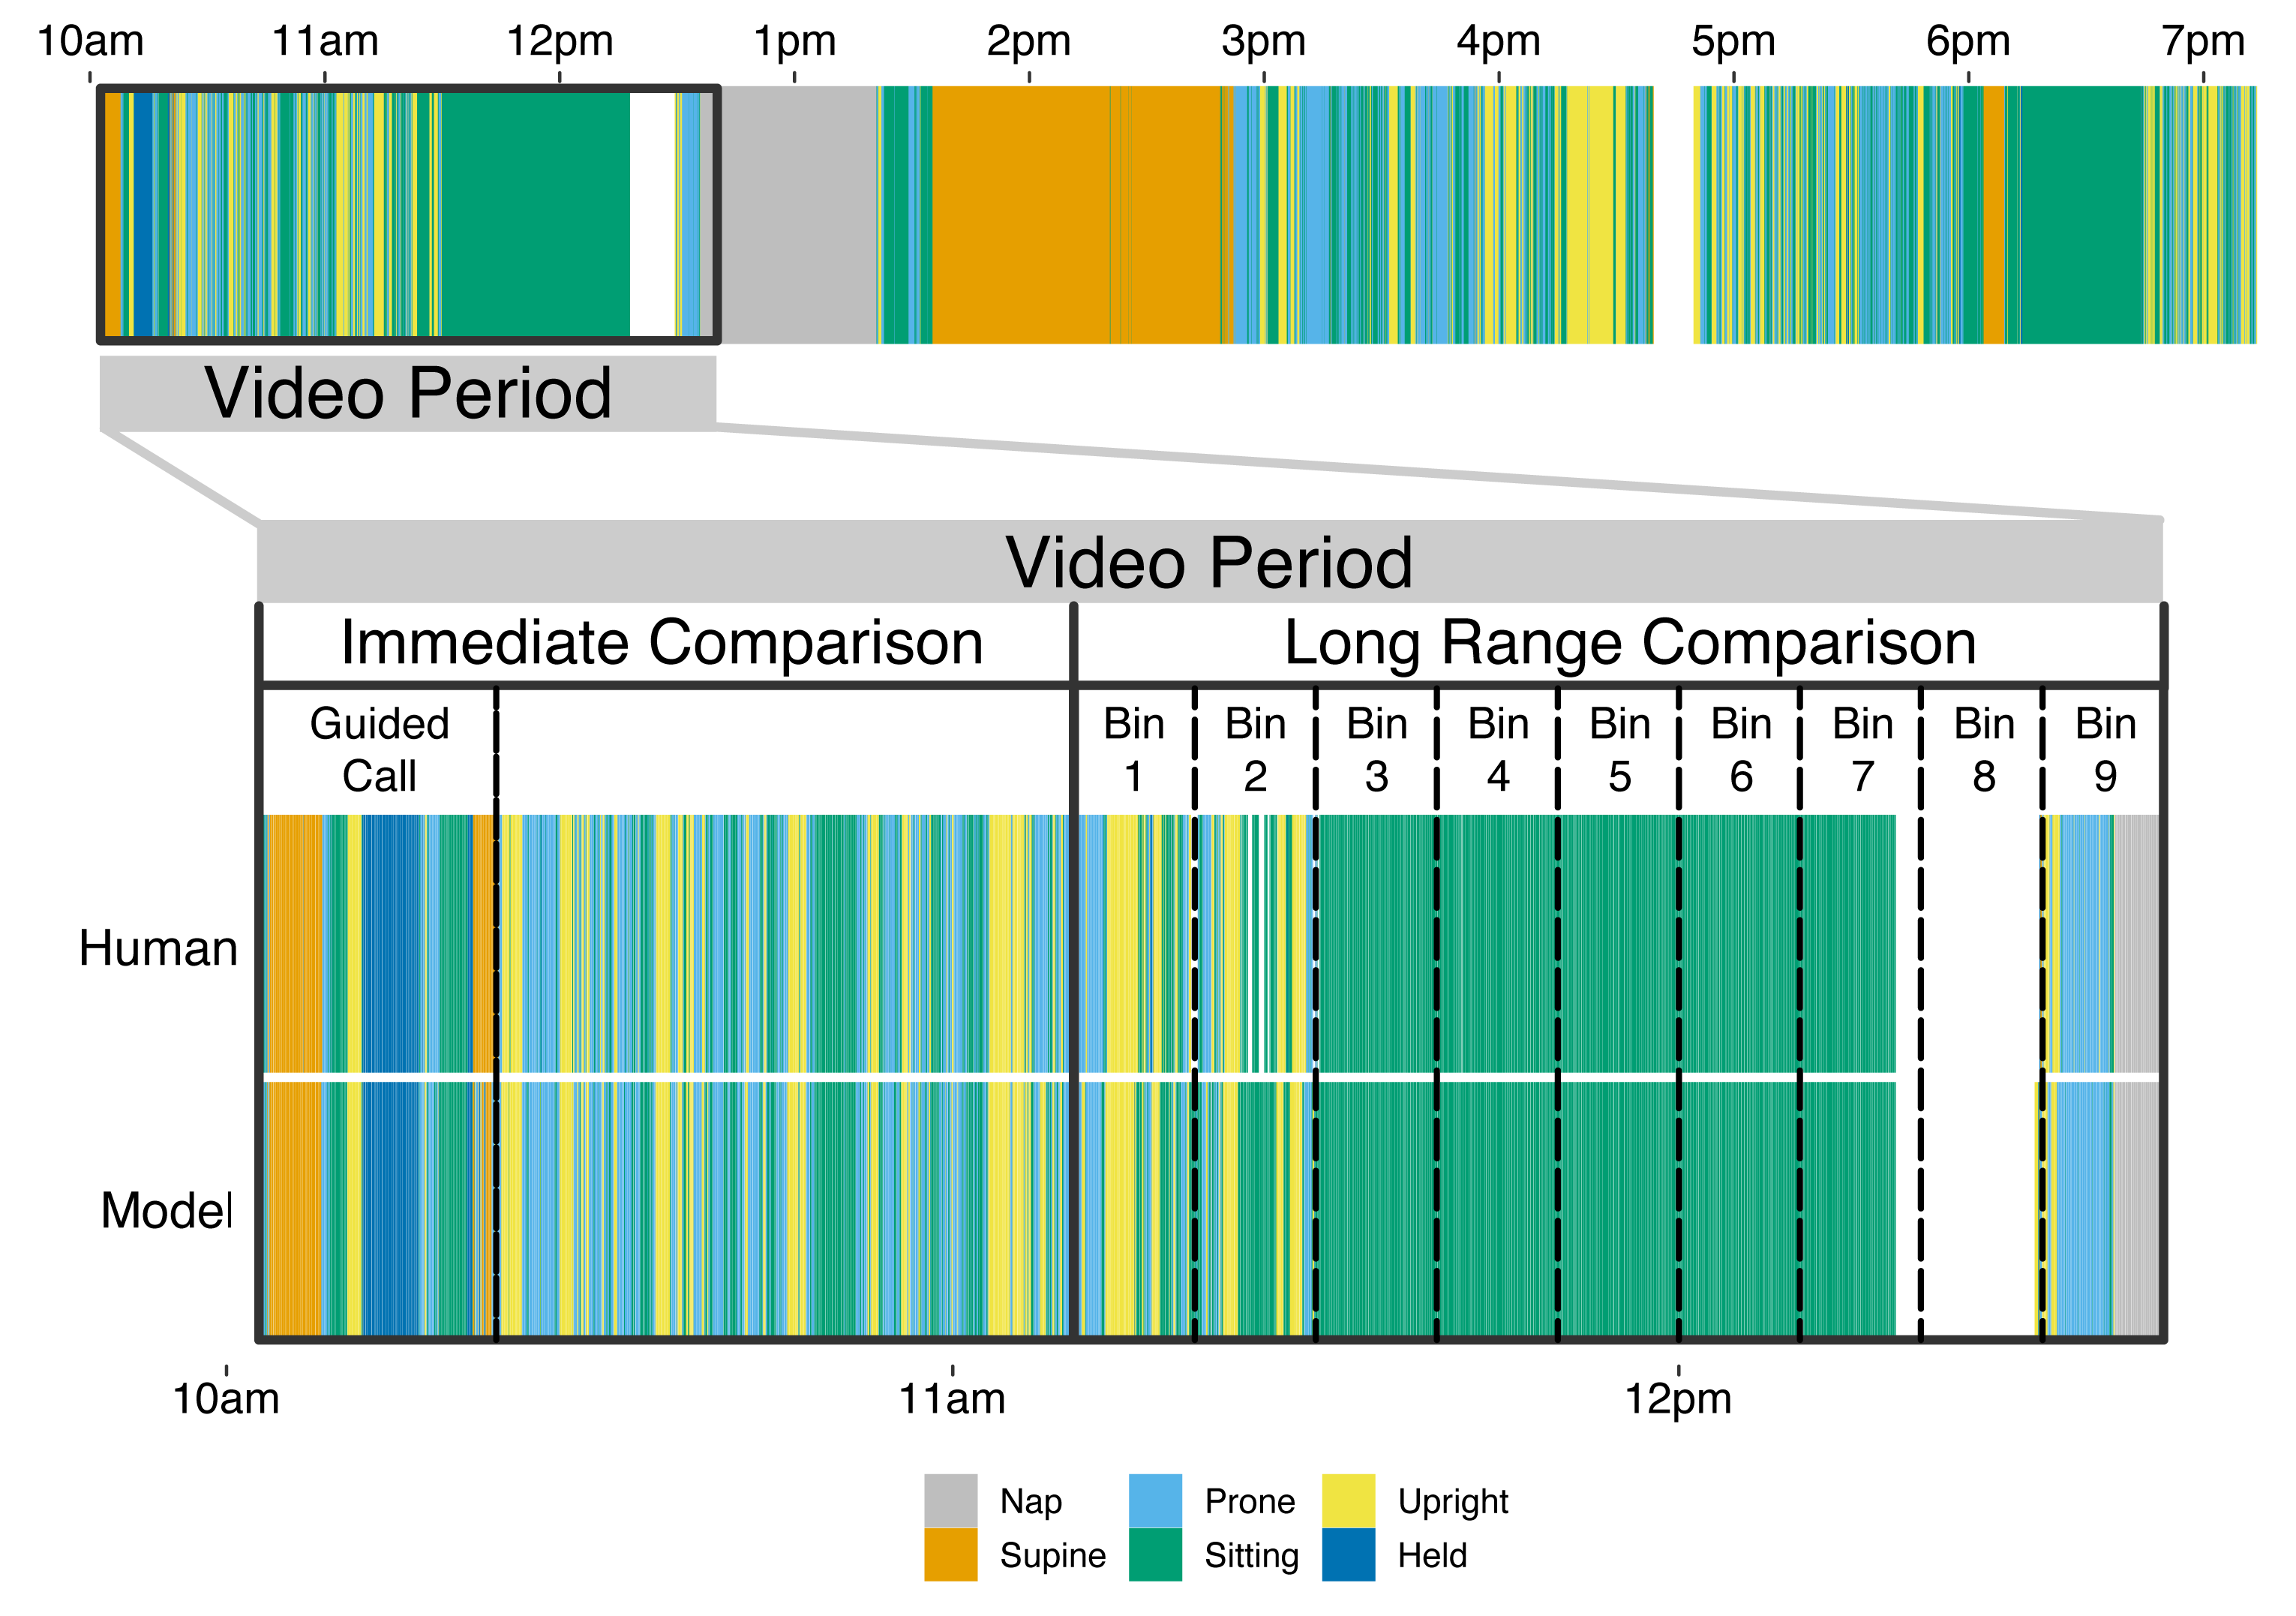
\includegraphics[width=0.99\linewidth]{figures/timeline} 

}

\caption{Example Timeline Caption.}\label{fig:exemplartimeline}
\end{figure}

\hypertarget{body-position-annotation}{%
\subsection{Body position annotation}\label{body-position-annotation}}

\hypertarget{body-position-classification}{%
\subsection{Body position classification}\label{body-position-classification}}

\hypertarget{results}{%
\section{Results}\label{results}}

\hypertarget{goal-1-assess-the-proximal-accuracy-of-body-position-classification-models}{%
\subsection{Goal 1: Assess the proximal accuracy of body position classification models}\label{goal-1-assess-the-proximal-accuracy-of-body-position-classification-models}}

\begin{figure}

{\centering 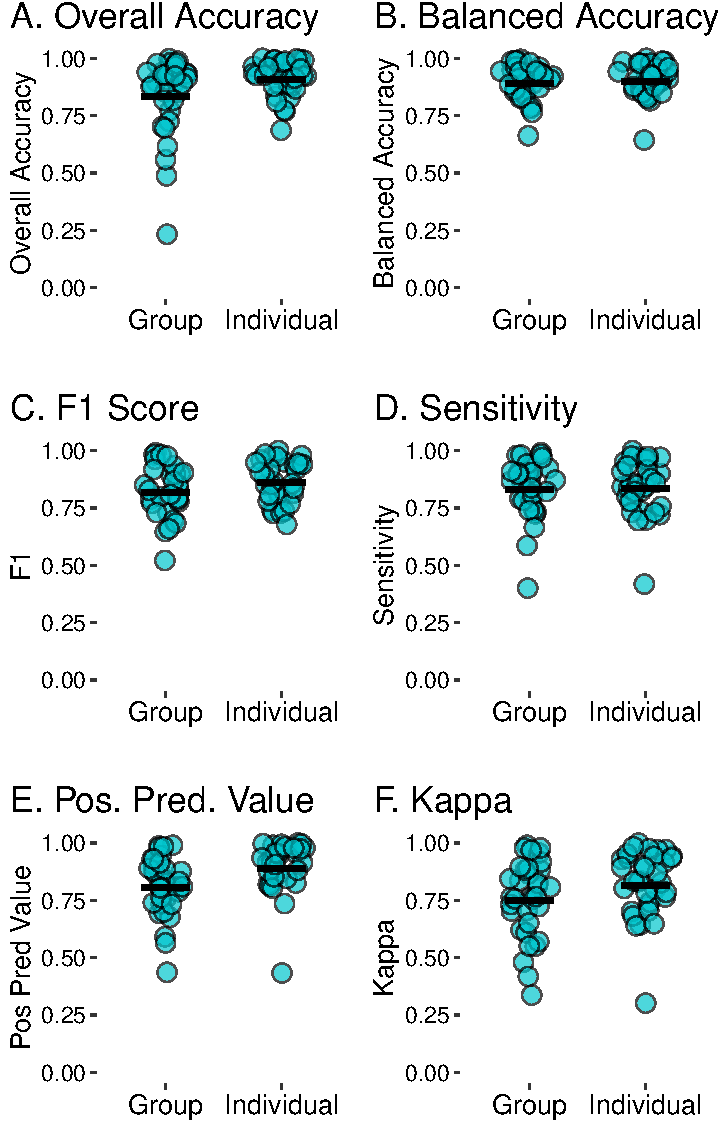
\includegraphics{manuscript_files/figure-latex/metrics-1} 

}

\caption{Metrics}\label{fig:metrics}
\end{figure}

\begin{table}[tbp]

\begin{center}
\begin{threeparttable}

\caption{\label{tab:metricstable}Summary statistics for model performance metrics shown separately for group and individual models.}

\begin{tabular}{lllllll}
\toprule
 & \multicolumn{3}{c}{Group} & \multicolumn{3}{c}{Individual} \\
\cmidrule(r){2-4} \cmidrule(r){5-7}
Metric & Median & Mean & SD & Median & Mean & SD\\
\midrule
Overall Accuracy & 0.908 & 0.848 & 0.143 & 0.936 & 0.919 & 0.071\\
Balanced Accuracy & 0.909 & 0.897 & 0.074 & 0.916 & 0.907 & 0.072\\
F1 & 0.813 & 0.827 & 0.101 & 0.873 & 0.870 & 0.089\\
Sensitivity & 0.840 & 0.836 & 0.123 & 0.848 & 0.840 & 0.121\\
Pos Pred Value & 0.822 & 0.815 & 0.125 & 0.915 & 0.899 & 0.108\\
Kappa & 0.769 & 0.757 & 0.160 & 0.846 & 0.820 & 0.141\\
\bottomrule
\end{tabular}

\end{threeparttable}
\end{center}

\end{table}

\renewcommand{\arraystretch}{.75}

\begin{table}[tbp]

\begin{center}
\begin{threeparttable}

\caption{\label{tab:metricsbyclass}Model performance metrics for each body position category, shown separately for group and individual models.}

\begin{tabular}{llllllll}
\toprule
 &  & \multicolumn{3}{c}{Group} & \multicolumn{3}{c}{Individual} \\
\cmidrule(r){3-5} \cmidrule(r){6-8}
Metric & Position & Median & Mean & SD & Median & Mean & SD\\
\midrule
Balanced Accuracy & Supine & 0.977 & 0.935 & 0.099 & 0.995 & 0.957 & 0.090\\
 & Prone & 0.997 & 0.950 & 0.110 & 0.983 & 0.921 & 0.132\\
 & Sitting & 0.932 & 0.861 & 0.151 & 0.973 & 0.943 & 0.071\\
 & Upright & 0.930 & 0.867 & 0.146 & 0.937 & 0.877 & 0.123\\
 & Held & 0.907 & 0.872 & 0.111 & 0.892 & 0.854 & 0.153\\ \midrule
F1 & Supine & 0.952 & 0.873 & 0.173 & 0.987 & 0.937 & 0.130\\
 & Prone & 0.965 & 0.923 & 0.124 & 0.958 & 0.889 & 0.186\\
 & Sitting & 0.897 & 0.805 & 0.247 & 0.963 & 0.927 & 0.101\\
 & Upright & 0.781 & 0.748 & 0.235 & 0.868 & 0.769 & 0.227\\
 & Held & 0.813 & 0.783 & 0.163 & 0.862 & 0.786 & 0.240\\ \midrule
Sensitivity & Supine & 1.000 & 0.945 & 0.125 & 1.000 & 0.948 & 0.141\\
 & Prone & 1.000 & 0.907 & 0.216 & 0.988 & 0.856 & 0.266\\
 & Sitting & 0.901 & 0.787 & 0.291 & 0.977 & 0.917 & 0.136\\
 & Upright & 0.878 & 0.767 & 0.275 & 0.893 & 0.790 & 0.255\\
 & Held & 0.867 & 0.774 & 0.229 & 0.817 & 0.722 & 0.309\\ \midrule
Pos Pred Value & Supine & 0.973 & 0.802 & 0.300 & 1.000 & 0.939 & 0.131\\
 & Prone & 0.991 & 0.896 & 0.196 & 0.993 & 0.901 & 0.197\\
 & Sitting & 0.910 & 0.840 & 0.238 & 0.967 & 0.947 & 0.078\\
 & Upright & 0.848 & 0.743 & 0.285 & 0.875 & 0.817 & 0.205\\
 & Held & 0.917 & 0.803 & 0.247 & 0.949 & 0.872 & 0.232\\ \midrule
Kappa & Supine & 0.932 & 0.770 & 0.307 & 0.984 & 0.913 & 0.169\\
 & Prone & 0.951 & 0.887 & 0.208 & 0.948 & 0.851 & 0.242\\
 & Sitting & 0.836 & 0.712 & 0.308 & 0.946 & 0.889 & 0.134\\
 & Upright & 0.729 & 0.700 & 0.277 & 0.829 & 0.744 & 0.232\\
 & Held & 0.786 & 0.733 & 0.219 & 0.845 & 0.744 & 0.280\\
\bottomrule
\end{tabular}

\end{threeparttable}
\end{center}

\end{table}

\hypertarget{goal-2-assess-the-distal-accuracy-of-body-position-classification-models}{%
\subsection{Goal 2: Assess the distal accuracy of body position classification models}\label{goal-2-assess-the-distal-accuracy-of-body-position-classification-models}}

\begin{figure}

{\centering 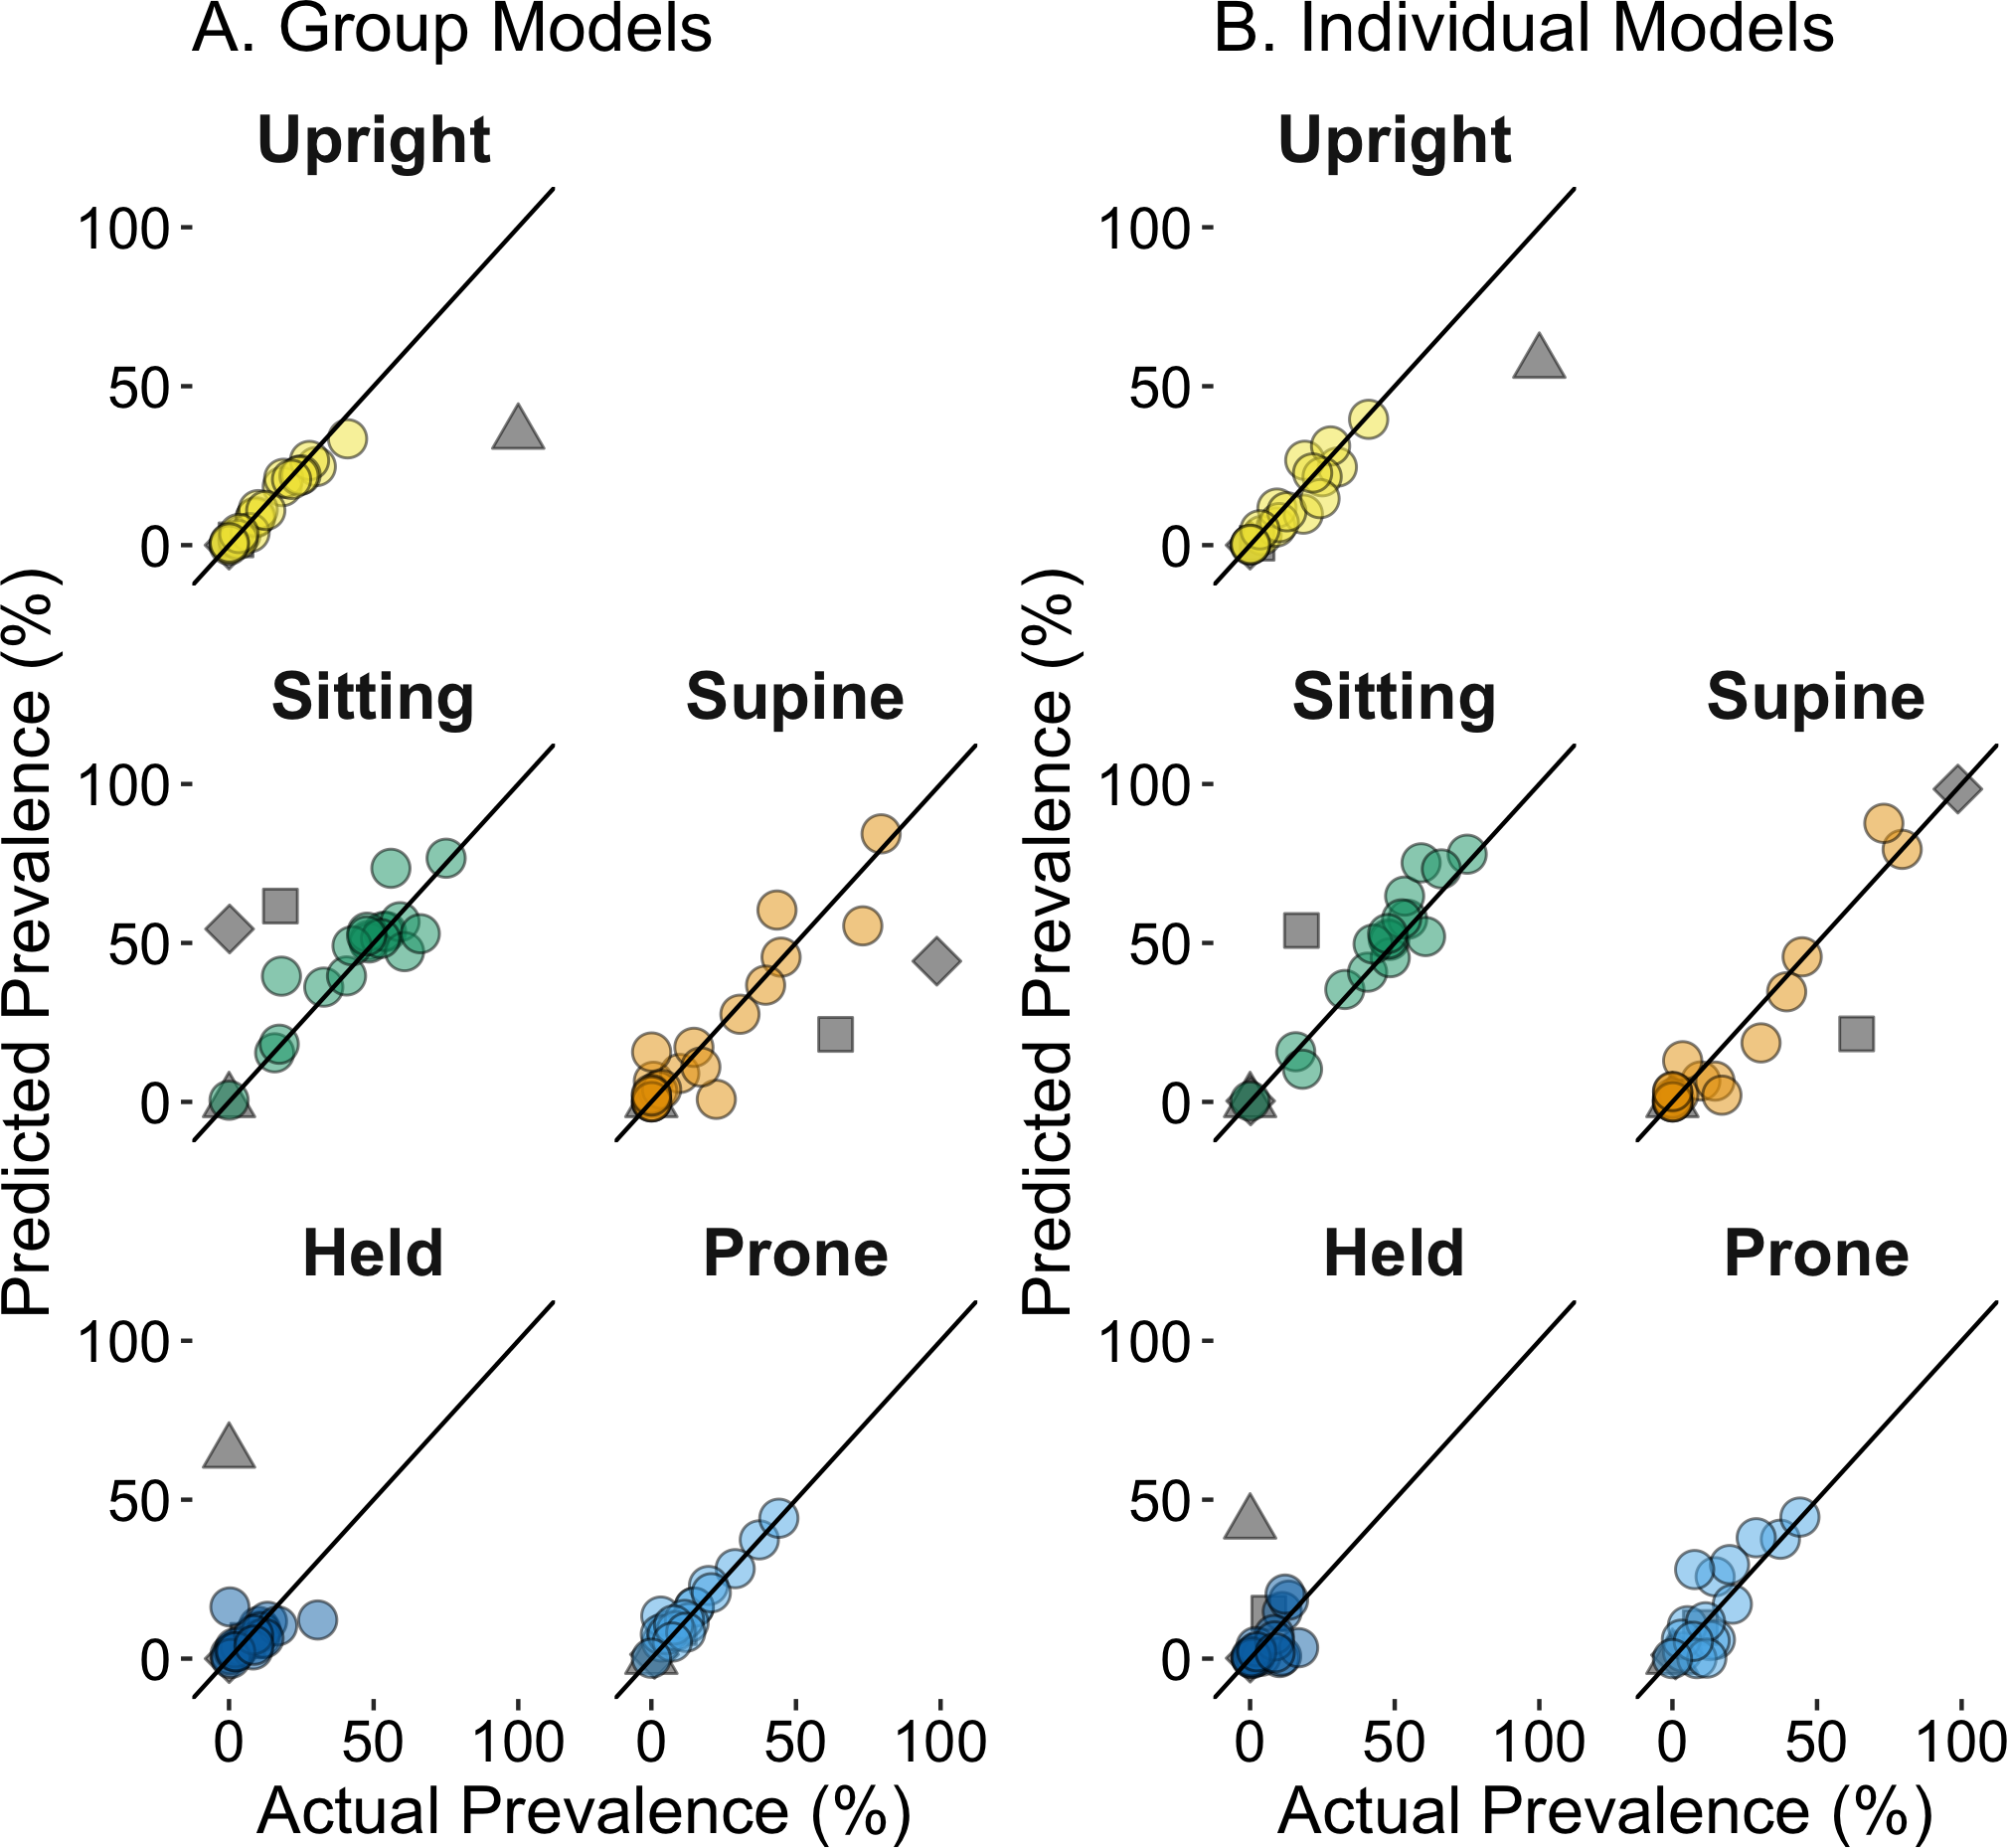
\includegraphics{manuscript_files/figure-latex/part2overall-1} 

}

\caption{Overall agreement between human-coded body position and model-predicted body position in the distal comparison. Agreement for group models is shown in (A) and agreement for individual models is shown in (B). Plots are shown separately for each body position with a reference line that indicates perfect agreement; each point in a plot represent data for a single participant. The three outlier participants are plotted in dark gray, with a different shape marking each individual.}\label{fig:part2overall}
\end{figure}

\begin{table}[tbp]

\begin{center}
\begin{threeparttable}

\caption{\label{tab:pt2overalltable}Correlations between human-coded and model-predicted body position durations across the entire long delay period. Correlations are provided within each posture and overall, and computed separately using group and individual models with and without outlier participants.}

\begin{tabular}{lllll}
\toprule
 & \multicolumn{2}{c}{With Outliers} & \multicolumn{2}{c}{Without Outliers} \\
\cmidrule(r){2-3} \cmidrule(r){4-5}
Position & Group & Individual & Group & Individual\\
\midrule
Held & -0.03 & 0.12 & 0.55 & 0.58\\
Prone & 0.97 & 0.85 & 0.97 & 0.84\\
Sitting & 0.73 & 0.93 & 0.91 & 0.97\\
Supine & 0.84 & 0.94 & 0.94 & 0.97\\
Upright & 0.84 & 0.93 & 0.99 & 0.94\\ \midrule
Overall & 0.80 & 0.91 & 0.95 & 0.96\\
\bottomrule
\end{tabular}

\end{threeparttable}
\end{center}

\end{table}

\begin{figure}

{\centering 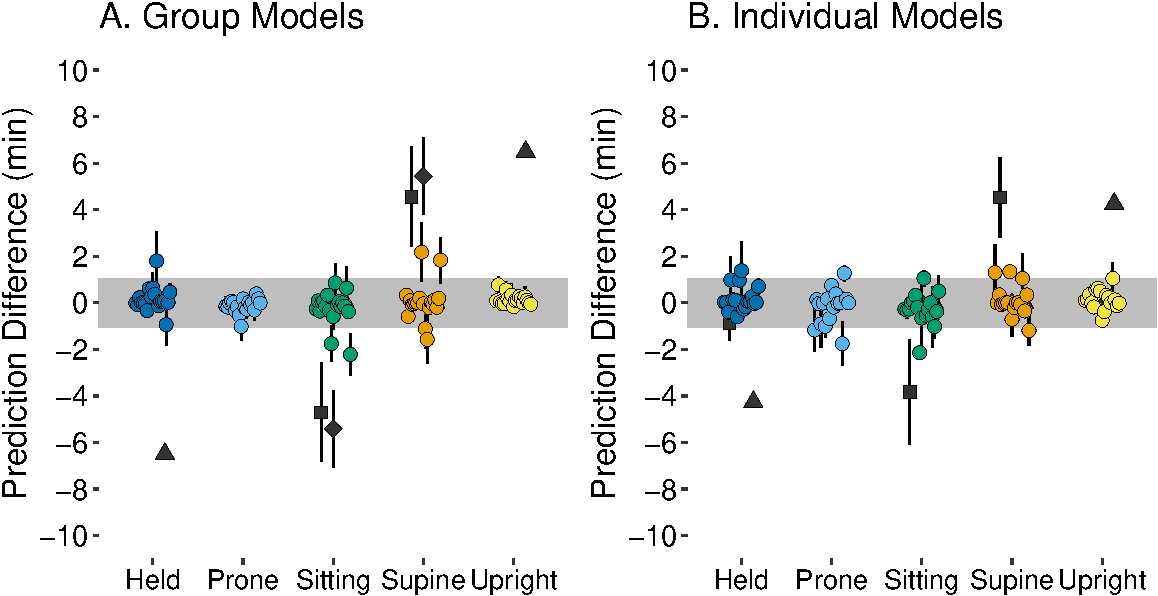
\includegraphics{manuscript_files/figure-latex/part2bins-1} 

}

\caption{Prediction performance (difference in minutes between human-coded and model-predicted body position) for 10-minute bins in the distal comparison. Each point shows the mean and SE for a single participant for each body position, summarizing the prediction difference for each of their 10-minute bins. Points falling within the gray shaded region indicate that average prediction errors were less than 1 minute. Performance is plotted separately for (A) group models and (B) individual models. The three outlier participants are plotted in dark gray, with a different shape marking each individual.}\label{fig:part2bins}
\end{figure}

\begin{table}[tbp]

\begin{center}
\begin{threeparttable}

\caption{\label{tab:pt2binstable}Correlations between human-coded and model-predicted body position durations using 10-minute bins during the distal comparison. Correlations are provided within each posture and overall, and computed separately using group and individual models with and without outlier participants.}

\begin{tabular}{lllll}
\toprule
 & \multicolumn{2}{c}{With Outliers} & \multicolumn{2}{c}{Without Outliers} \\
\cmidrule(r){2-3} \cmidrule(r){4-5}
Position & Group & Individual & Group & Individual\\
\midrule
Held & 0.45 & 0.43 & 0.57 & 0.55\\
Prone & 0.96 & 0.89 & 0.96 & 0.88\\
Sitting & 0.72 & 0.92 & 0.91 & 0.93\\
Supine & 0.75 & 0.95 & 0.90 & 0.94\\
Upright & 0.93 & 0.95 & 0.97 & 0.95\\ \midrule
Overall & 0.80 & 0.94 & 0.93 & 0.94\\
\bottomrule
\end{tabular}

\end{threeparttable}
\end{center}

\end{table}

\hypertarget{goal-3-examine-the-data-quality-of-full-day-home-recordings}{%
\subsection{Goal 3: Examine the data quality of full-day home recordings}\label{goal-3-examine-the-data-quality-of-full-day-home-recordings}}

\begin{figure}

{\centering 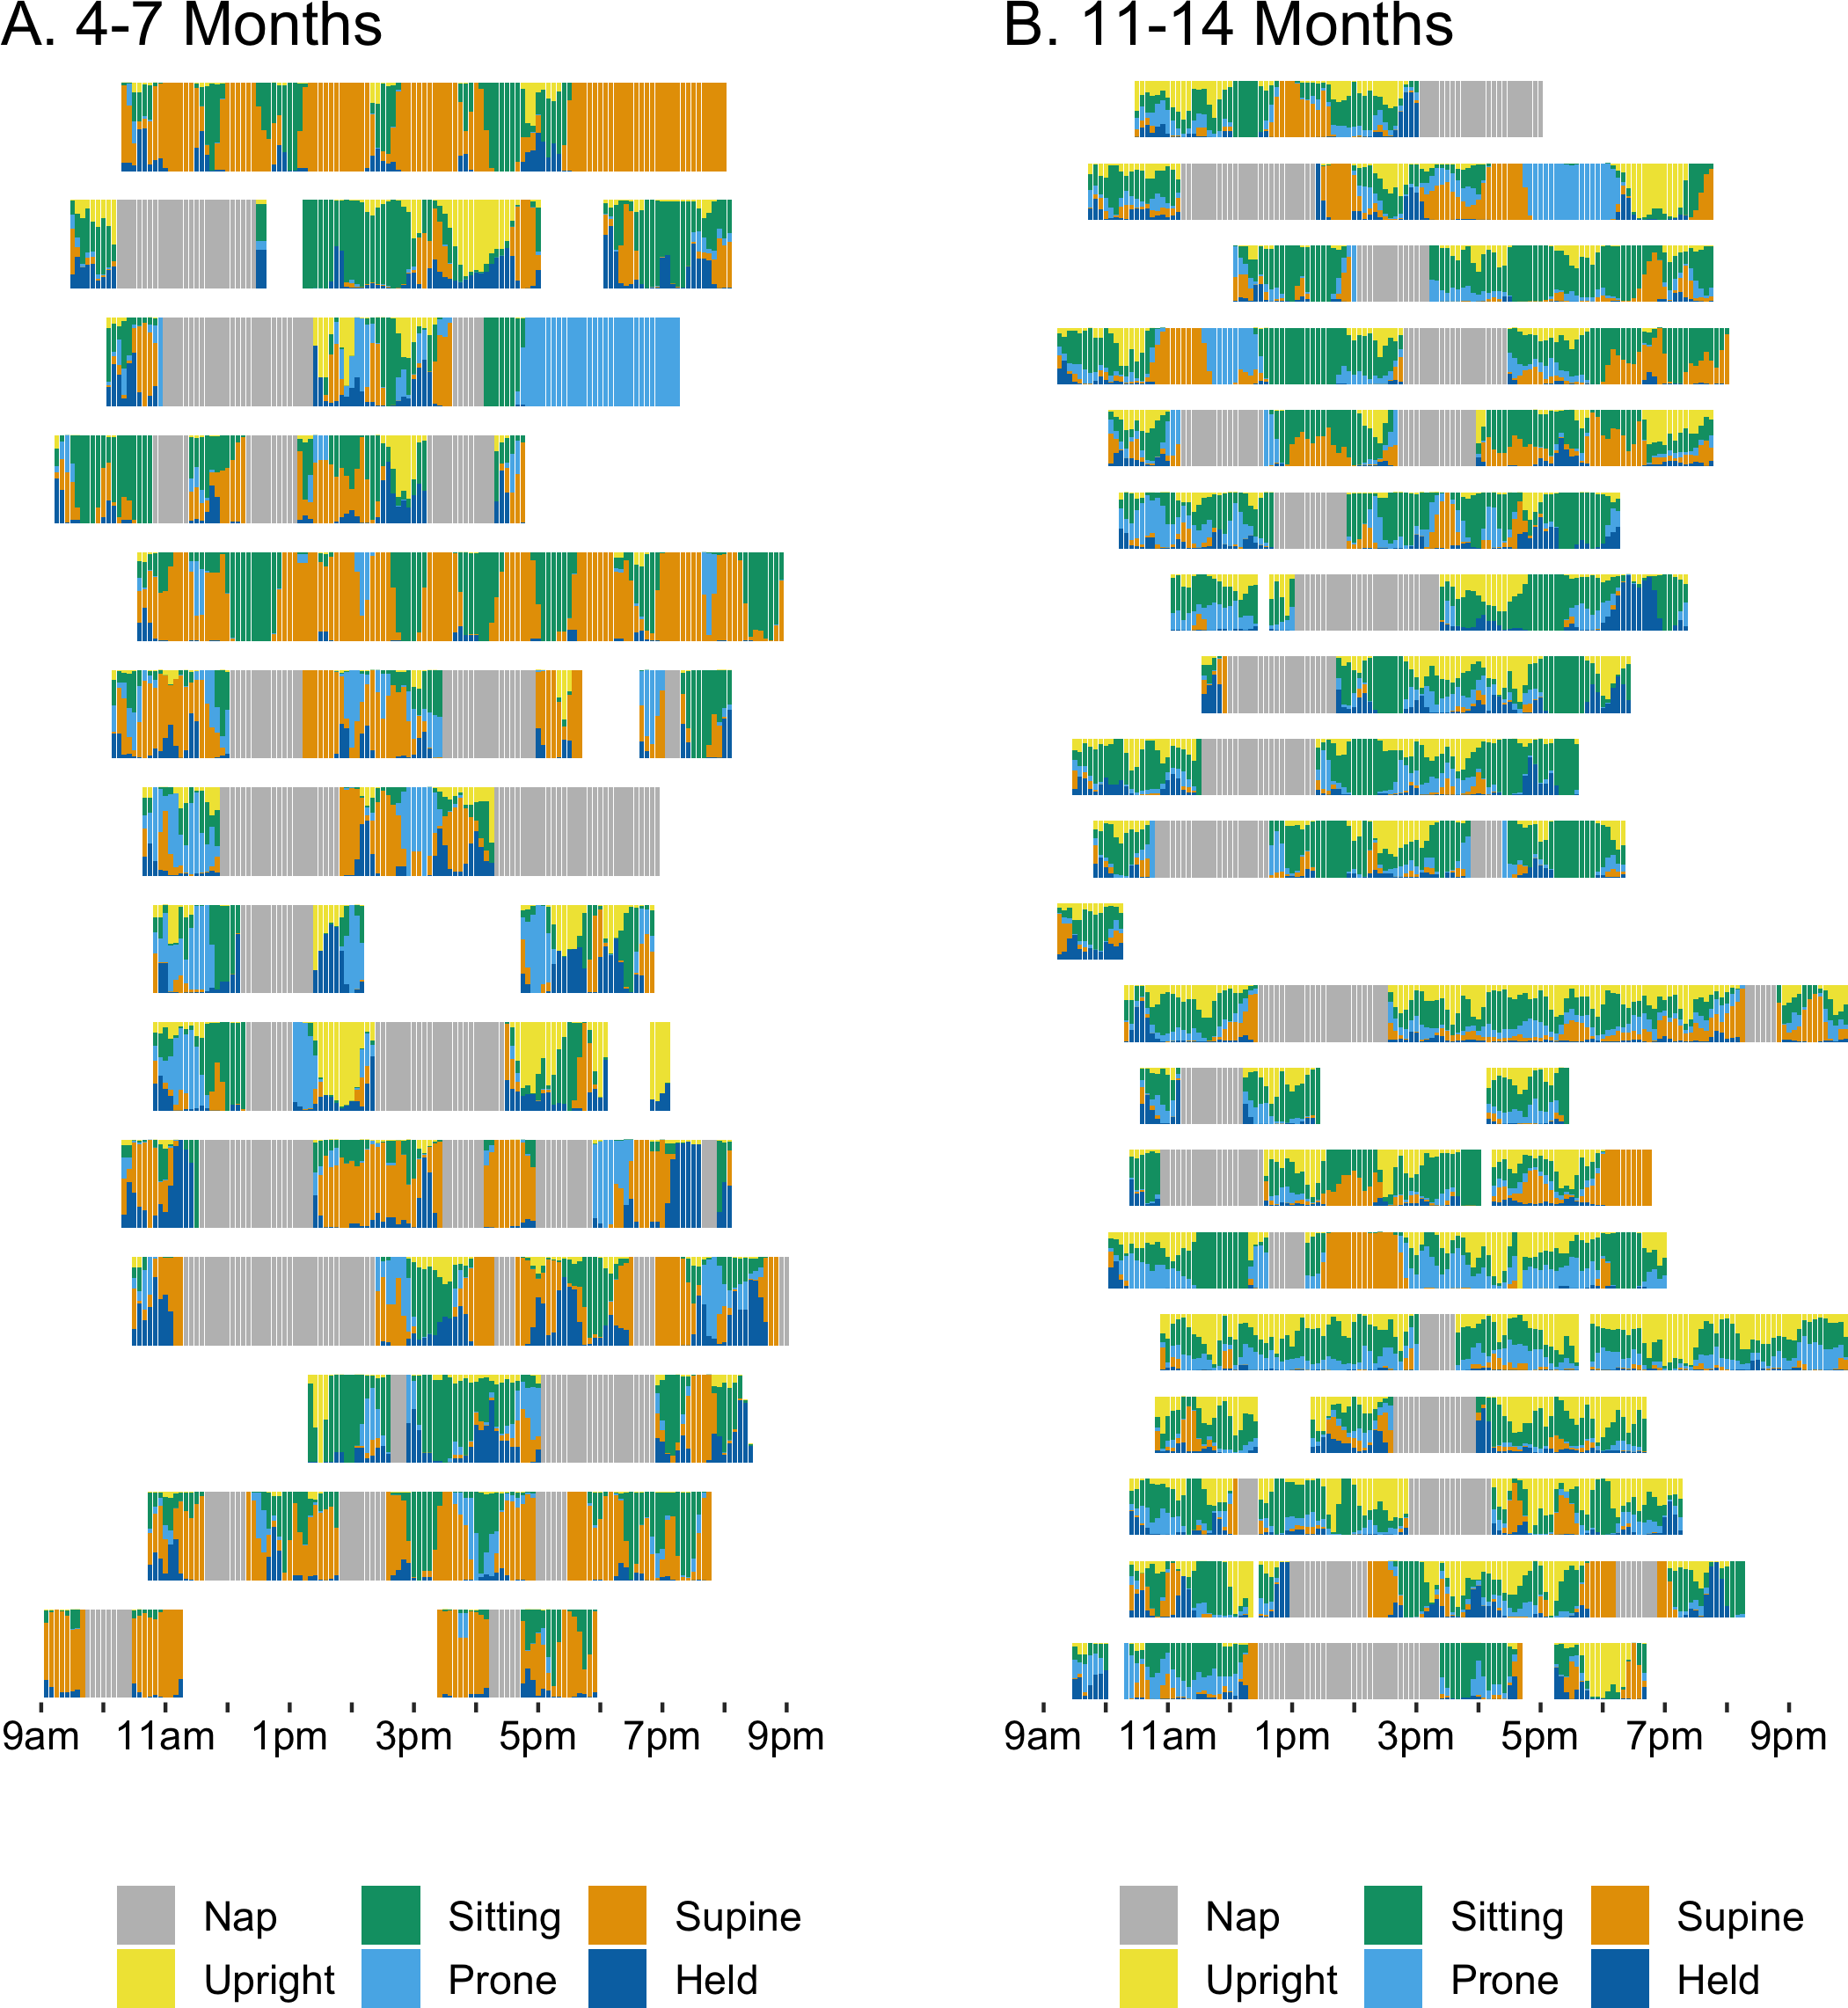
\includegraphics{manuscript_files/figure-latex/timelines-1} 

}

\caption{Timelines}\label{fig:timelines}
\end{figure}

\hypertarget{goal-4-assess-the-suitability-of-full-day-predictions-for-capturing-age-differences-in-body-position}{%
\subsection{Goal 4: Assess the suitability of full-day predictions for capturing age differences in body position}\label{goal-4-assess-the-suitability-of-full-day-predictions-for-capturing-age-differences-in-body-position}}

\begin{figure}

{\centering 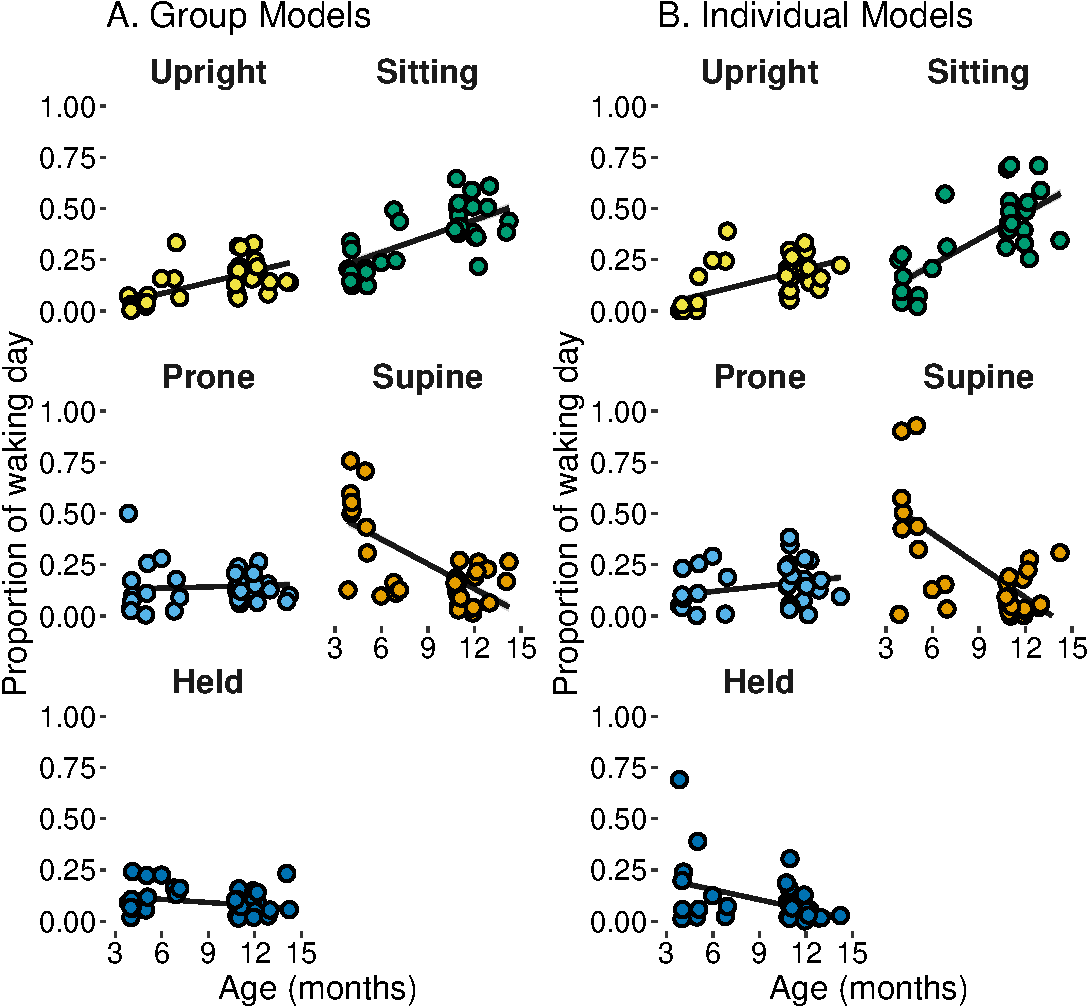
\includegraphics{manuscript_files/figure-latex/age-1} 

}

\caption{Age trends}\label{fig:age}
\end{figure}

\begin{table}[tbp]

\begin{center}
\begin{threeparttable}

\caption{\label{tab:agetable}Summary of age differences in full-day body position for younger (4- to 7-month) and older (11- to 14-month) infants. Values shown are the mean percent of time for each body position averaged across infants in each group. Standard deviations are shown in parentheses. Descriptive statistics are shown separately for group and individual models.}

\begin{tabular}{lllll}
\toprule
 & \multicolumn{2}{c}{Group} & \multicolumn{2}{c}{Individual} \\
\cmidrule(r){2-3} \cmidrule(r){4-5}
Position & Younger & Older & Younger & Older\\
\midrule
Upright & 7.6\% (8.9) & 18.6\% (7.4) & 9.9\% (13.1) & 18.7\% (8.4)\\
Sitting & 26.3\% (12.1) & 44.4\% (10.1) & 20.2\% (16.3) & 46.9\% (13.3)\\
Prone & 13.8\% (13.5) & 14.4\% (6.0) & 11.9\% (9.9) & 16.9\% (10.6)\\
Supine & 37.9\% (23.2) & 14.0\% (8.4) & 39.4\% (30.3) & 10.0\% (9.5)\\
Held & 12.7\% (6.9) & 8.5\% (5.4) & 17.6\% (19.9) & 7.4\% (7.6)\\
\bottomrule
\end{tabular}

\end{threeparttable}
\end{center}

\end{table}

\hypertarget{discussion}{%
\section{Discussion}\label{discussion}}

\newpage

\hypertarget{references}{%
\section{References}\label{references}}

\hypertarget{refs}{}
\begin{CSLReferences}{1}{0}
\leavevmode\vadjust pre{\hypertarget{ref-AdolphCTL2014}{}}%
Adolph, K. E., \& Tamis-LeMonda, C. S. (2014). The costs and benefits of development: The transition from crawling to walking. \emph{Child Development Perspectives}, \emph{8}, 187--192. \url{https://doi.org/10.1111/cdep.12085}

\leavevmode\vadjust pre{\hypertarget{ref-AiraksinenRasanen2020}{}}%
Airaksinen, M., Räsänen, O., Ilén, E., Häyrinen, T., Kivi, A., Marchi, V., Gallen, A., Blom, S., Varhe, A., Kaartinen, N., et al. (2020). Automatic posture and movement tracking of infants with wearable movement sensors. \emph{Scientific Reports}, \emph{10}(1), 1--13.

\leavevmode\vadjust pre{\hypertarget{ref-BarbaroFausey2022}{}}%
Barbaro, K. de, \& Fausey, C. M. (2022). Ten lessons about infants' everyday experiences. \emph{Current Directions in Psychological Science}, \emph{31}(1), 28--33. \url{https://doi.org/10.1177/09637214211059536}

\leavevmode\vadjust pre{\hypertarget{ref-Bergelson2019Input}{}}%
Bergelson, E., Amatuni, A., Dailey, S., Koorathota, S., \& Tor, S. (2019). Day by day, hour by hour: Naturalistic language input to infants. \emph{Developmental Science}, \emph{22}, e12715.

\leavevmode\vadjust pre{\hypertarget{ref-Bergelson2019Corpus}{}}%
Bergelson, E., Casillas, M., Soderstrom, M., Seidl, A., Warlaumont, A. S., \& Amatuni, A. (2019). What do {N}orth {A}merican babies hear? {A} large-scale cross-corpus analysis. \emph{Developmental Science}, \emph{22}, e12724.

\leavevmode\vadjust pre{\hypertarget{ref-ChenSchneider2022}{}}%
Chen, Q., Schneider, J. L., West, K. L., \& Iverson, J. M. (2022). Infant locomotion shapes proximity to adults during everyday play in the u.s. \emph{Infancy}. \url{https://doi.org/10.1111/infa.12503}

\leavevmode\vadjust pre{\hypertarget{ref-CristiaLavechin2020}{}}%
Cristia, A., Lavechin, M., Scaff, C., Soderstrom, M., Rowland, C., Räsänen, O., Bunce, J., \& Bergelson, E. (2020). A thorough evaluation of the language environment analysis ({LENA}) system. \emph{Behavior Research Methods}, \emph{53}(2), 467--486. \url{https://doi.org/10.3758/s13428-020-01393-5}

\leavevmode\vadjust pre{\hypertarget{ref-Survey}{}}%
Franchak, J. M. (2019). Changing opportunities for learning in everyday life: Infant body position over the first year. \emph{Infancy}, \emph{24}, 187--209.

\leavevmode\vadjust pre{\hypertarget{ref-Freeplay}{}}%
Franchak, J. M., Kretch, K. S., \& Adolph, K. E. (2018). See and be seen: Infant-caregiver social looking during locomotor free play. \emph{Developmental Science}, \emph{21}, e12626.

\leavevmode\vadjust pre{\hypertarget{ref-GallandTaylor2012}{}}%
Galland, B. C., Taylor, B. J., Elder, D. E., \& Herbison, P. (2012). Normal sleep patterns in infants and children: A systematic review of observational studies. \emph{Sleep Medicine Reviews}, \emph{16}(3), 213--222. \url{https://doi.org/10.1016/j.smrv.2011.06.001}

\leavevmode\vadjust pre{\hypertarget{ref-Karasik2011}{}}%
Karasik, L. B., Tamis-LeMonda, C. S., \& Adolph, K. E. (2011). Transition from crawling to walking and infants' actions with objects and people. \emph{Child Development}, \emph{82}, 1199--1209. \url{https://doi.org/10.1111/j.1467-8624.2011.01595.x}

\leavevmode\vadjust pre{\hypertarget{ref-Karasik2014}{}}%
Karasik, L. B., Tamis-LeMonda, C. S., \& Adolph, K. E. (2014). Crawling and walking infants elicit different verbal responses from mothers. \emph{Developmental Science}, \emph{17}, 388--395. \url{https://doi.org/10.1111/desc.12129}

\leavevmode\vadjust pre{\hypertarget{ref-CWW}{}}%
Kretch, K. S., Franchak, J. M., \& Adolph, K. E. (2014). Crawling and walking infants see the world differently. \emph{Child Development}, \emph{85}, 1503--1518. \url{https://doi.org/10.1111/cdev.12206}

\leavevmode\vadjust pre{\hypertarget{ref-LuoFranchak2020}{}}%
Luo, C., \& Franchak, J. M. (2020). Head and body structure infants' visual experiences during mobile, naturalistic play. \emph{{PLoS ONE}}, \emph{15}, e0242009.

\leavevmode\vadjust pre{\hypertarget{ref-MalachowskiSalo2023}{}}%
Malachowski, L. G., Salo, V. C., Needham, A. W., \& Humphreys, K. L. (2023). Infant placement and language exposure in daily life. \emph{Infant and Child Development}. \url{https://doi.org/10.1002/icd.2405}

\leavevmode\vadjust pre{\hypertarget{ref-MendozaFausey2021}{}}%
Mendoza, J. K., \& Fausey, C. M. (2021). Everyday music in infancy. \emph{Developmental Science}, \emph{24}(6). \url{https://doi.org/10.1111/desc.13122}

\leavevmode\vadjust pre{\hypertarget{ref-MendozaFausey2022}{}}%
Mendoza, J. K., \& Fausey, C. M. (2022). Everyday parameters for episode-to-episode dynamics in the daily music of infancy. \emph{Cognitive Science}, \emph{46}(8). \url{https://doi.org/10.1111/cogs.13178}

\leavevmode\vadjust pre{\hypertarget{ref-MichelettiYao2022}{}}%
Micheletti, M., Yao, X., Johnson, M., \& Barbaro, K. de. (2022). Validating a model to detect infant crying from naturalistic audio. \emph{Behavior Research Methods}. \url{https://doi.org/10.3758/s13428-022-01961-x}

\leavevmode\vadjust pre{\hypertarget{ref-PerryPrince2018}{}}%
Perry, L. K., Prince, E. B., Valtierra, A. M., Rivero-Fernandez, C., Ullery, M. A., Katz, L. F., Laursen, B., \& Messinger, D. S. (2018). A year in words: The dynamics and consequences of language experiences in an intervention classroom. \emph{{PLOS} {ONE}}, \emph{13}(7), e0199893. \url{https://doi.org/10.1371/journal.pone.0199893}

\leavevmode\vadjust pre{\hypertarget{ref-RasanenSeshadri2020}{}}%
Räsänen, O., Seshadri, S., Lavechin, M., Cristia, A., \& Casillas, M. (2020). {ALICE}: An open-source tool for automatic measurement of phoneme, syllable, and word counts from child-centered daylong recordings. \emph{Behavior Research Methods}, \emph{53}(2), 818--835. \url{https://doi.org/10.3758/s13428-020-01460-x}

\leavevmode\vadjust pre{\hypertarget{ref-SoskaAdolph2014}{}}%
Soska, K. C., \& Adolph, K. E. (2014). Postural position constrains multimodal object exploration in infants. \emph{Infancy}, \emph{19}, 138--161. \url{https://doi.org/10.1111/infa.12039}

\leavevmode\vadjust pre{\hypertarget{ref-Thurman2017}{}}%
Thurman, S. L., \& Corbetta, D. (2017). Spatial exploration and changes in infant-mother dyads around transitions in infant locomotion. \emph{Developmental Psychology}, \emph{53}, 1207--1221.

\leavevmode\vadjust pre{\hypertarget{ref-WarlaumontSobowale2021}{}}%
Warlaumont, A. S., Sobowale, K., \& Fausey, C. M. (2021). Daylong mobile audio recordings reveal multitimescale dynamics in infants' vocal productions and auditory experiences. \emph{Current Directions in Psychological Science}, \emph{31}(1), 12--19. \url{https://doi.org/10.1177/09637214211058166}

\leavevmode\vadjust pre{\hypertarget{ref-WassPhillips2022}{}}%
Wass, S., Phillips, E., Smith, C., Fatimehin, E. O., \& Goupil, L. (2022). Vocal communication is tied to interpersonal arousal coupling in caregiver-infant dyads. \emph{{eLife}}, \emph{11}. \url{https://doi.org/10.7554/elife.77399}

\leavevmode\vadjust pre{\hypertarget{ref-Weisleder2013}{}}%
Weisleder, A., \& Fernald, A. (2013). Talking to children matters: Early language experience strengthens processing and builds vocabulary. \emph{Psychological Science}, \emph{24}, 2143--2152.

\leavevmode\vadjust pre{\hypertarget{ref-WestIverson2021}{}}%
West, K. L., \& Iverson, J. M. (2021). Communication changes when infants begin to walk. \emph{Developmental Science}, \emph{24}(5). \url{https://doi.org/10.1111/desc.13102}

\end{CSLReferences}


\end{document}
